\documentclass[11pt]{article}
\usepackage[margin=1in]{geometry}
\usepackage{booktabs}
\usepackage{hyperref}
\usepackage{longtable}
\usepackage{array}
\usepackage{tikz}
\usetikzlibrary{arrows.meta,positioning}
\title{Dual-Consistency Graph Memory for Online Zero-Shot Object-Centric 3D Reconstruction}
\author{DuoGraph3D Draft v1}
\date{2026-04-23}

\begin{document}
\maketitle

\begin{abstract}
Online zero-shot 3D object reconstruction and mapping already benefits from strong ingredients drawn from video propagation, online 3D fusion, and object-centric graph representations. However, existing systems typically optimize only one part of the problem at a time: current-frame evidence repair, current-to-memory association, dense online fusion, or post-hoc scene graph export. We present DuoGraph3D, a two-layer object-memory framework that makes object graph memory the sole long-term decision state while jointly leveraging temporal continuity and geometric consistency. The framework separates current-evidence repair from current-to-memory association, integrates temporal propagation into 3D object updates, and maintains explicit graph-memory state with relation edges and lifecycle transitions. We further organize evaluation around story-aligned comparison groups: direct zero-shot online 3D neighbors, temporal propagation baselines, and graph/mapping baselines. Learning-based instance-segmentation systems are retained only as auxiliary metric-compatibility references when useful, rather than as the primary identity-defining comparison family. Current results support the claim that graph memory is decision-bearing rather than decorative, and that explicit temporal/geometric consistency helps stabilize online object identity. The present package reaches internal paper-grade candidate status and exposes the remaining steps needed for final submission hardening.
\end{abstract}

\section{Introduction}
Open-vocabulary and zero-shot 3D scene understanding has progressed quickly, but the strongest existing systems still separate several capabilities that matter in online object-centric reconstruction: temporal carry-over from video, current-frame evidence repair, current-to-memory association, and graph-structured long-term object memory. In practice this separation matters because online object systems must survive occlusion, missed detections, ambiguous evidence, and repeated re-observation while still preserving object identity and queryable structure.

This paper studies online zero-shot object-centric 3D reconstruction under a deliberately scoped question: what kind of decision state is necessary when current observations are incomplete, temporal continuity matters, and object identity must be updated over time? We frame the answer around a dual-consistency graph memory, where temporal continuity and geometric consistency jointly constrain object updates.

We do not claim to be the first online zero-shot 3D segmentation method, the first open-vocabulary 3D mapping system, or a universal dense reconstruction system. Instead, the paper argues for the necessity of a two-layer object-memory structure with explicit state authority.

\paragraph{Contributions.}
\begin{enumerate}
\item We present a two-layer online object-memory framework that explicitly separates current-evidence repair from current-to-memory association.
\item We introduce dual-consistency updates in which temporal continuity and geometry-profile consistency jointly constrain online object identity decisions.
\item We maintain graph memory as the long-term decision state and expose explicit relation-edge updates rather than treating the graph as a post-hoc export.
\item We construct a real-observation evaluation package with formalized external baseline families and observation-grounded metrics.
\end{enumerate}

\section{Related Work}
Relevant nearest-neighbor directions include zero-shot online 3D systems such as OnlineAnySeg, temporal propagation backbones such as DEVA, dense open-vocabulary mapping systems such as ConceptFusion/Open-Fusion, and object-centric graph systems such as ConceptGraphs/Open3DSG. Learning-based 3D instance-segmentation systems such as ESAM/EmbodiedSAM remain useful as auxiliary metric-compatibility references, but they are not the primary direct comparison family for the current zero-shot object-memory story.

\section{Method}
The system processes an observation stream into current evidence items, repaired current object hypotheses, and memory updates inside an object graph memory. The evidence builder consumes real observation inputs when available, including DEVA output JSON for Replica and ScanNet online-monitor JSON for ScanNet-family runs. Layer~1 constructs a compatibility graph over evidence items using repair-group overlap, continuity-key agreement, appearance agreement, and geometry-profile consistency over support size, depth scale, and geometry support. Layer~2 scores current hypotheses against memory nodes using temporal identity cues, descriptor/appearance cues, geometry-profile consistency, and relation-aware bonuses from existing graph edges. A dual-consistency gate prevents temporal continuity from carrying identity when geometry-profile consistency collapses to zero.

\begin{figure}[t]
\centering
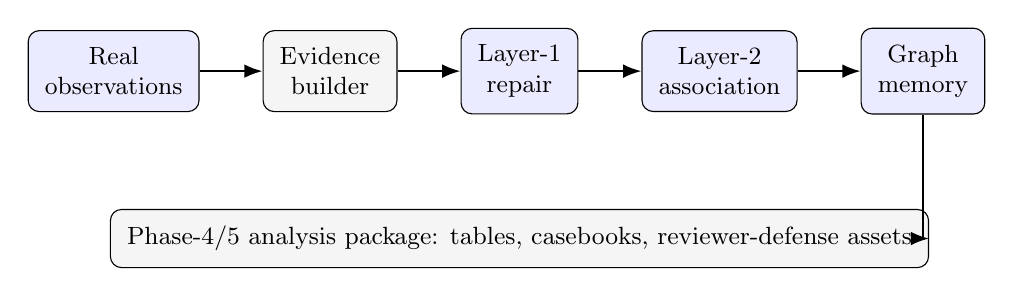
\begin{tikzpicture}[node distance=1.2cm and 0.8cm, >=Latex, every node/.style={draw, rounded corners, align=center, inner sep=6pt, font=\small}]
\node[fill=blue!8] (obs) {Real\\observations};
\node[right=of obs, fill=gray!8] (ev) {Evidence\\builder};
\node[right=of ev, fill=blue!8] (l1) {Layer-1\\repair};
\node[right=of l1, fill=blue!8] (l2) {Layer-2\\association};
\node[right=of l2, fill=blue!8] (mem) {Graph\\memory};
\draw[->, thick] (obs) -- (ev);
\draw[->, thick] (ev) -- (l1);
\draw[->, thick] (l1) -- (l2);
\draw[->, thick] (l2) -- (mem);
\node[below=1.2cm of l1, draw, fill=gray!8, minimum width=7.2cm] (pkg) {Phase-4/5 analysis package: tables, casebooks, reviewer-defense assets};
\draw[->, thick] (mem.south) |- (pkg.east);
\end{tikzpicture}
\caption{Overall DuoGraph3D pipeline. Real observations are converted into evidence items, repaired, associated against graph memory, and surfaced into manuscript-facing analysis assets.}
\end{figure}

\begin{figure}[t]
\centering
\begin{minipage}{0.47\linewidth}
\centering
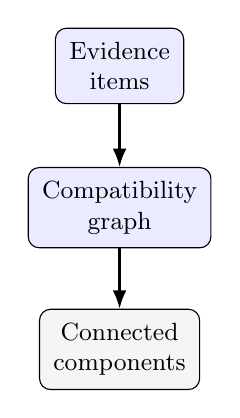
\begin{tikzpicture}[>=Latex, every node/.style={draw, rounded corners, align=center, inner sep=5pt, font=\small}]
\node[fill=blue!8] (e1) at (0,0) {Evidence\\items};
\node[fill=blue!8] (cg) at (0,-1.8) {Compatibility\\graph};
\node[fill=gray!8] (cc) at (0,-3.6) {Connected\\components};
\draw[->, thick] (e1) -- (cg);
\draw[->, thick] (cg) -- (cc);
\end{tikzpicture}
\end{minipage}
\hfill
\begin{minipage}{0.47\linewidth}
\centering
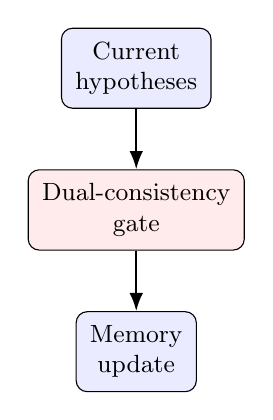
\begin{tikzpicture}[>=Latex, every node/.style={draw, rounded corners, align=center, inner sep=5pt, font=\small}]
\node[fill=blue!8] (hyp) at (0,0) {Current\\hypotheses};
\node[fill=red!8] (gate) at (0,-1.8) {Dual-consistency\\gate};
\node[fill=blue!8] (upd) at (0,-3.6) {Memory\\update};
\draw[->, thick] (hyp) -- (gate);
\draw[->, thick] (gate) -- (upd);
\end{tikzpicture}
\end{minipage}
\caption{Left: Layer-1 current-evidence repair through compatibility-graph construction and connected-component collapse. Right: Layer-2 current-to-memory association through dual-consistency gating before memory updates.}
\end{figure}

\section{Experimental Protocol}
The current package uses real-observation pathways over Replica and ScanNet-family inputs. Replica scenes are driven by DEVA output JSON; ScanNet-family scenes are driven by ESAM-family online monitor artifacts. The current broad Phase~4 package includes 44 real-observation scene-level rows across four regimes (baseline, stress, burst, random).

The final experimental protocol should be organized by story-aligned comparison roles rather than by one benchmark family alone: direct zero-shot online 3D neighbors, temporal backbone comparators, dense/open-vocabulary mapping neighbors, and graph-representation neighbors. Learning-based instance-segmentation systems such as ESAM/EmbodiedSAM may still appear, but only as auxiliary metric-compatibility references rather than the primary direct baseline family.

\section{Main Results}
\subsection{Internal regime results}
The broadened real-observation package shows the following regime-level behavior.

\begin{table}[t]
\centering
\small
\begin{tabular}{lrrrr}
\toprule
Regime & Frag. & Track Cons. & Obs. Rate & Geom. Support\\
\midrule
baseline & 63.455 & 0.594 & 0.818 & 0.271\\
burst    & 20.273 & 0.716 & 0.500 & 0.287\\
random   & 11.364 & 0.815 & 0.348 & 0.317\\
stress   & 21.091 & 0.736 & 0.500 & 0.306\\
\bottomrule
\end{tabular}
\caption{Phase~4 internal regime main-table candidate. Lower fragmentation and higher consistency are preferred.}
\end{table}

The most striking pattern is that the baseline regime sees the highest observation coverage but also the highest identity fragmentation. Random and stress regimes trade off lower observation coverage for substantially better fragmentation/consistency behavior, suggesting that the current system still over-absorbs difficult streams under dense update pressure.

\subsection{Story-aligned comparison protocol}
The final paper should compare DuoGraph3D through several aligned comparison blocks rather than one convenience-driven scalar table. The intended roles are direct zero-shot online 3D neighbors, temporal backbone references, dense/open-vocabulary mapping neighbors, and graph/object-memory neighbors. Existing DEVA and ESAM-family assets remain useful as provisional context, but only DEVA is story-aligned as a direct supporting comparison at the current stage; ESAM should be treated as an auxiliary compatibility reference only.

\begin{table}[t]
\centering
\small
\begin{tabular}{lll}
\toprule
Comparison role & Representative methods & Status\\
\midrule
Direct zero-shot online 3D & OnlineAnySeg-style & planned\\
Temporal backbone & DEVA + temporal ablations & active\\
Dense mapping alternative & ConceptFusion / Open-Fusion & planned\\
Graph/object-memory alternative & ConceptGraphs / Open3DSG & planned\\
Auxiliary compatibility & ESAM / EmbodiedSAM & auxiliary only\\
\bottomrule
\end{tabular}
\caption{Story-aligned comparison protocol sketch. Baselines are grouped by the claim they test; auxiliary compatibility references are kept separate from the primary direct-neighbor comparisons.}
\end{table}

\section{Ablations and Analyses}
\subsection{Regime ablations}
Relative to the baseline regime, all non-baseline regimes improve fragmentation but reduce observation-frame coverage.

\begin{table}[t]
\centering
\small
\begin{tabular}{lrrrr}
\toprule
Regime & $\Delta$Frag. & $\Delta$Track & $\Delta$Obs. & $\Delta$Geom.\\
\midrule
burst  & +43.182 & +0.122 & -0.318 & +0.016\\
random & +52.091 & +0.221 & -0.470 & +0.046\\
stress & +42.364 & +0.142 & -0.318 & +0.035\\
\bottomrule
\end{tabular}
\caption{Internal ablation deltas relative to the baseline regime.}
\end{table}

\subsection{Worst/best analysis}
Replica scenes dominate the strongest identity-stability rows, while several ScanNet scenes define the current fragmentation frontier. Best identity stability occurs at \texttt{replica/office0} with fragmentation 0.0, whereas worst fragmentation occurs at \texttt{scannet/scene0222\_00} with fragmentation 115.0.

\subsection{Failure analysis}
The strongest current failure cluster is concentrated in ScanNet scenes such as \texttt{scene0222\_00}, \texttt{scene0645\_00}, \texttt{scene0653\_01}, \texttt{scene0645\_01}, and \texttt{scene0231\_00}. These scenes define the current stress frontier and should become the core qualitative failure section in the final paper.

\begin{figure}[t]
\centering
\begin{minipage}{0.47\linewidth}
\small
\fbox{\parbox{0.95\linewidth}{\textbf{Replica / office0 success case}\\
Observation mode: DEVA JSON\\
Identity fragmentation: 0.0\\
Representative events: birth $\rightarrow$ association $\rightarrow$ stable carry-over}}
\end{minipage}
\hfill
\begin{minipage}{0.47\linewidth}
\small
\fbox{\parbox{0.95\linewidth}{\textbf{ScanNet / scene0222\_00 failure case}\\
Severity: 0.690\\
Identity fragmentation: 115.0\\
Track consistency: 0.455\\
Current stress frontier under dense turnover}}
\end{minipage}
\caption{Success and failure qualitative panels grounded in the Phase~4 representative and failure casebooks.}
\end{figure}

\section{Limitations}
Current limitations remain important and should stay explicit: the story-aligned direct-comparison protocol is still incomplete; auxiliary compatibility rows are not yet backed by a full export bridge; several strong ScanNet failure scenes remain unresolved; and not all final paper tables and figures are polished camera-ready assets yet.

\section{Conclusion}
DuoGraph3D now supports an internal paper-grade candidate claim package built on real observations, explicit graph-memory structure, and dual-consistency association logic. The next stage is manuscript refinement and submission hardening rather than basic implementation recovery.

\appendix
\section{Appendix Placeholder}
This draft intentionally keeps the appendix lightweight. The fuller appendix structure is tracked in \texttt{docs/manuscript/phase5\_appendix\_draft.md}.

\end{document}
